%%
%% This is file `sample-sigconf.tex',
%% generated with the docstrip utility.
%%
%% The original source files were:
%%
%% samples.dtx  (with options: `all,proceedings,bibtex,sigconf')
%% 
%% IMPORTANT NOTICE:
%% 
%% For the copyright see the source file.
%% 
%% Any modified versions of this file must be renamed
%% with new filenames distinct from sample-sigconf.tex.
%% 
%% For distribution of the original source see the terms
%% for copying and modification in the file samples.dtx.
%% 
%% This generated file may be distributed as long as the
%% original source files, as listed above, are part of the
%% same distribution. (The sources need not necessarily be
%% in the same archive or directory.)
%%
%%
%% Commands for TeXCount
%TC:macro \cite [option:text,text]
%TC:macro \citep [option:text,text]
%TC:macro \citet [option:text,text]
%TC:envir table 0 1
%TC:envir table* 0 1
%TC:envir tabular [ignore] word
%TC:envir displaymath 0 word
%TC:envir math 0 word
%TC:envir comment 0 0
%%
%% The first command in your LaTeX source must be the \documentclass
%% command.
%%
%% For submission and review of your manuscript please change the
%% command to \documentclass[manuscript, screen, review]{acmart}.
%%
%% When submitting camera ready or to TAPS, please change the command
%% to \documentclass[sigconf]{acmart} or whichever template is required
%% for your publication.
%%
%%
%\documentclass[sigconf]{acmart}
\documentclass[sigconf, review]{acmart}
%%
%% \BibTeX command to typeset BibTeX logo in the docs
\AtBeginDocument{%
  \providecommand\BibTeX{{%
    Bib\TeX}}}

%% Rights management information.  This information is sent to you
%% when you complete the rights form.  These commands have SAMPLE
%% values in them; it is your responsibility as an author to replace
%% the commands and values with those provided to you when you
%% complete the rights form.
\setcopyright{acmlicensed}
\copyrightyear{2018}
\acmYear{2018}
\acmDOI{XXXXXXX.XXXXXXX}
%% These commands are for a PROCEEDINGS abstract or paper.
\acmConference[Conference acronym 'XX]{Make sure to enter the correct
  conference title from your rights confirmation email}{June 03--05,
  2018}{Woodstock, NY}
%%
%%  Uncomment \acmBooktitle if the title of the proceedings is different
%%  from ``Proceedings of ...''!
%%
%%\acmBooktitle{Woodstock '18: ACM Symposium on Neural Gaze Detection,
%%  June 03--05, 2018, Woodstock, NY}
\acmISBN{978-1-4503-XXXX-X/2018/06}


%%
%% Submission ID.
%% Use this when submitting an article to a sponsored event. You'll
%% receive a unique submission ID from the organizers
%% of the event, and this ID should be used as the parameter to this command.
%%\acmSubmissionID{123-A56-BU3}

%%
%% For managing citations, it is recommended to use bibliography
%% files in BibTeX format.
%%
%% You can then either use BibTeX with the ACM-Reference-Format style,
%% or BibLaTeX with the acmnumeric or acmauthoryear sytles, that include
%% support for advanced citation of software artefact from the
%% biblatex-software package, also separately available on CTAN.
%%
%% Look at the sample-*-biblatex.tex files for templates showcasing
%% the biblatex styles.
%%

%%
%% The majority of ACM publications use numbered citations and
%% references.  The command \citestyle{authoryear} switches to the
%% "author year" style.
%%
%% If you are preparing content for an event
%% sponsored by ACM SIGGRAPH, you must use the "author year" style of
%% citations and references.
%% Uncommenting
%% the next command will enable that style.
%%\citestyle{acmauthoryear}

\usepackage{graphicx}
\usepackage{amsmath, amssymb}
\usepackage{hyperref}
\usepackage{cite}
\usepackage{algorithm}
\usepackage{algorithmic}
\usepackage{hyperref}
\usepackage{caption}
\usepackage{graphicx}
\graphicspath{ {./images/} }
\usepackage{booktabs} % For better table formatting
\usepackage{multirow} % For multirow cells
\usepackage{array} % For custom column alignment
\usepackage{tabularx} % For auto-adjusting table width
\usepackage{booktabs} % For better table formatting
\usepackage{adjustbox} % For scaling the table
\usepackage{geometry} % For better page margins
\usepackage{array}
\usepackage{rotating}


%%
%% end of the preamble, start of the body of the document source.
\begin{document}

%%
%% The "title" command has an optional parameter,
%% allowing the author to define a "short title" to be used in page headers.
\title{Analyzing Public Sentiment on Controversial Sports Events in YouTube Comments}

%%
%% The "author" command and its associated commands are used to define
%% the authors and their affiliations.
%% Of note is the shared affiliation of the first two authors, and the
%% "authornote" and "authornotemark" commands
%% used to denote shared contribution to the research.
\author{Yuvraj Singh}
%\authornote{Both authors contributed equally to this research.}
% \email{trovato@corporation.com}
% \orcid{1234-5678-9012}
% \author{G.K.M. Tobin}
% \authornotemark[1]

\affiliation{%
  \institution{IIIT Bhubaneswar}
  \city{Bhubaneswar, Orissa}
  %\state{Ohio}
  \country{India}
}
\email{yuvraj.mist@gmail.com}

\author{Devadripta Jadhav}
\affiliation{%
  \institution{Savitribai Phule Pune University}
  \city{Pune, Maharashtra}
  \country{India}}
\email{devadripta@gmail.com}

\author{Samiksha Boduwar}
\affiliation{%
  \institution{Savitribai Phule Pune University}
  \city{Pune, Maharashtra}
  \country{India}}
\email{samikshaboduwar@gmail.com}




\author{Kripabandhu Ghosh}
\affiliation{%
  \institution{IISER Kolkata}
  \city{Mohanpur, West Bengal}
  \country{India}}
\email{kripaghosh@iiserkol.ac.in}

%%
%% By default, the full list of authors will be used in the page
%% headers. Often, this list is too long, and will overlap
%% other information printed in the page headers. This command allows
%% the author to define a more concise list
%% of authors' names for this purpose.
\renewcommand{\shortauthors}{Yuvraj et al.}

%%
%% The abstract is a short summary of the work to be presented in the
%% article.
\begin{abstract}
  This paper presents an analysis of YouTube comments on famous and controversial Public Sports Events. We explore public stance (stance detection) on a total of 6 famous controversial sports incidents by extracting and processing YouTube comments. Stance detection is performed on multiple events, including \textit{The Underarm Incident}, \textit{Jonny Bairstow's Run-Out} Incident, \textit{Ashwin's Mankadding} Event, \textit{Luis Suarez Handball} Event etc. 
The complete event details,  results and evaluation metrics will be discussed in detail in subsequent sections.
\end{abstract}

%%
%% The code below is generated by the tool at http://dl.acm.org/ccs.cfm.
%% Please copy and paste the code instead of the example below.
%%
\begin{CCSXML}
<ccs2012>
   <concept>
       <concept_id>10002951.10003260.10003277</concept_id>
       <concept_desc>Information systems~Web mining</concept_desc>
       <concept_significance>500</concept_significance>
       </concept>
 </ccs2012>
\end{CCSXML}

\ccsdesc[500]{Information systems~Web mining}
%%
%% Keywords. The author(s) should pick words that accurately describe
%% the work being presented. Separate the keywords with commas.
\keywords{Stance Detection, YouTube Comments, Social Media Analysis, Sports Controversies}
%% A "teaser" image appears between the author and affiliation
%% information and the body of the document, and typically spans the
%% page.
% \begin{teaserfigure}
%   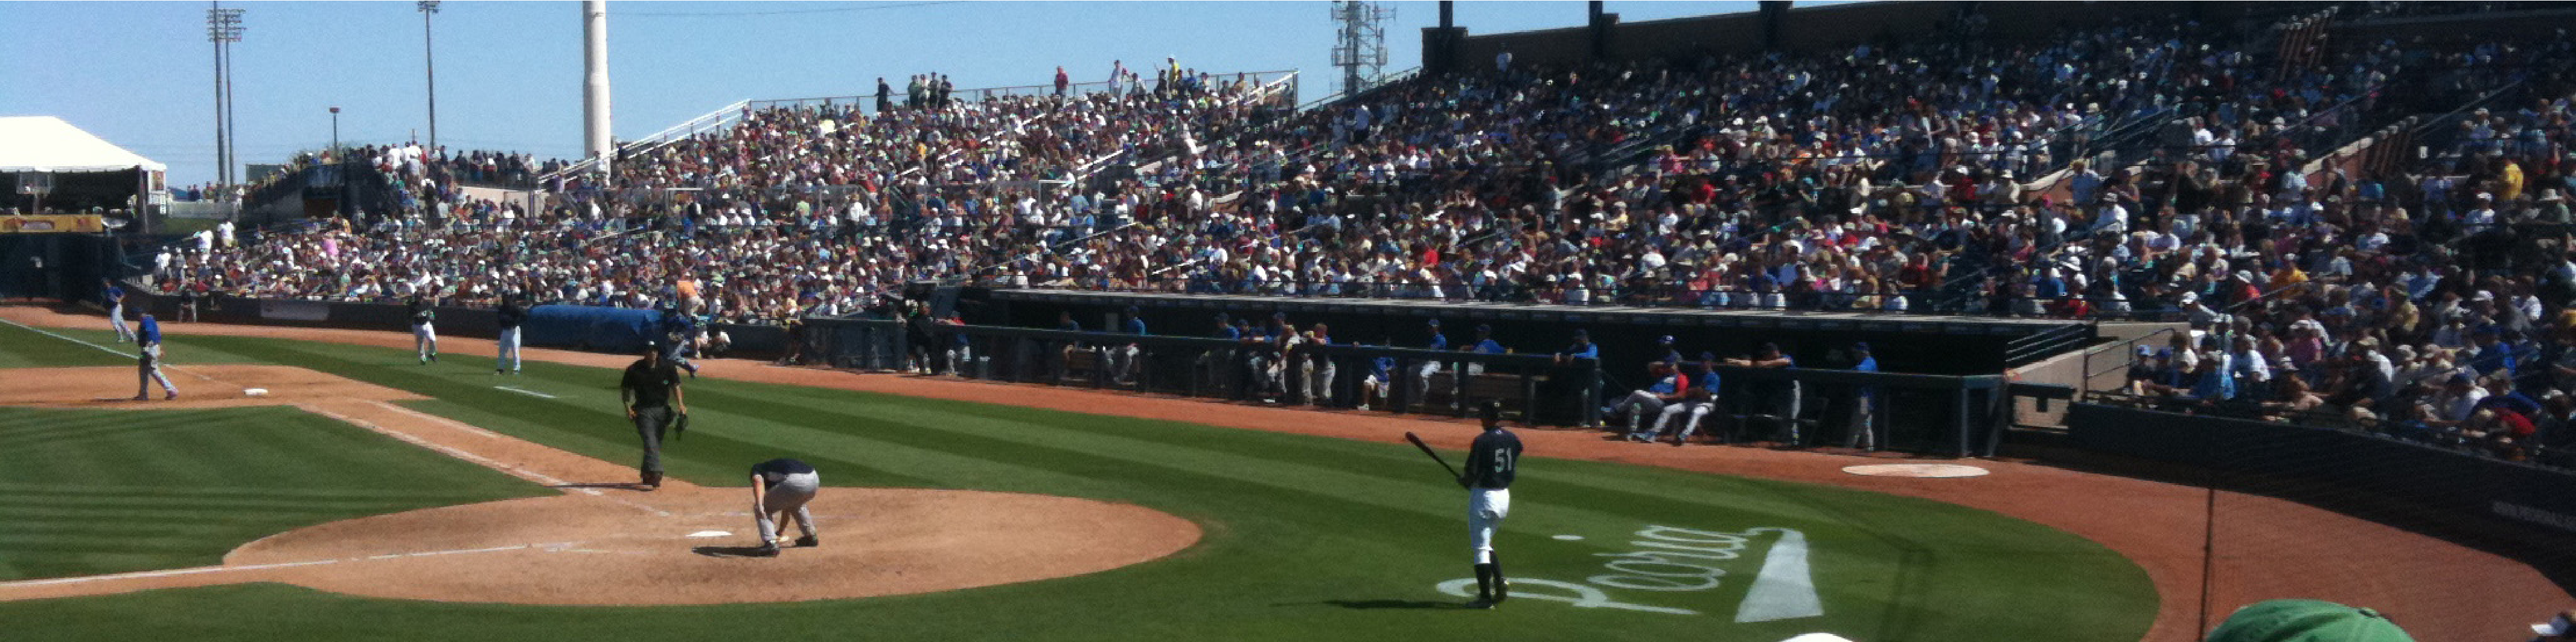
\includegraphics[width=\textwidth]{sampleteaser}
%   \caption{Seattle Mariners at Spring Training, 2010.}
%   \Description{Enjoying the baseball game from the third-base
%   seats. Ichiro Suzuki preparing to bat.}
%   \label{fig:teaser}
% \end{teaserfigure}

% \received{20 February 2007}
% \received[revised]{12 March 2009}
% \received[accepted]{5 June 2009}

%%
%% This command processes the author and affiliation and title
%% information and builds the first part of the formatted document.
\maketitle

\section{Introduction}
Sports engages billions of followers worldwide\footnote{\url{https://www.statista.com/chart/14329/global-interest-in-football/}} and impacts the economy %\cite{sportseconomics20221}. 
Sports controversies often ignite passionate discussions among fans, analysts, and players. With the rise of social media, platforms like YouTube have become central to these discussions. This study aims to analyze the stances or perform opinion mining namely for, against, and neutral on comments from famous social media platforms like YouTube, focusing on events such as Jonny Bairstow's Run-Out Incident, Luis Suarez Handball Event etc.
To our knowledge, the first-ever study of civic engagement in controversial sports events (cricket and football) spans around 40 years. LLMs (Llama3 family) were used for initial annotations (stance) of comments and later fine-tuned for comparative performance analysis ($~$30\% boost in accuracy).~\cite{Lamport:LaTeX}



Thereafter, a humanely verified dataset of 30,000 thousand comments is released. %\cite{sportqa}
{\color{red}KRIPA: Cite these https://aclanthology.org/search/?q=sports and explain why our work is different}

\section{Methodology}



\subsection{Data Collection}
{\color{red} First write about the six events in brief and state why did you choose these events (they had many comments, they span across a long duration of time, are from two very popular sports in the world and covering multiple continents.}
We identified YouTube videos related to each controversy based on quality and engagement (on average $>$ 5k comments) metrics. Our methodology focussed on the creation of a curated playlist for each event, ensuring diverse opinions.

The data extraction process involved:
\begin{enumerate}
    \item Identifying a famous public sports controversy from relevant sources like YouTube, Wikipedia and news sources based on quality and engagement.
    \item Identifying relevant videos for the chosen public sports controversies.
    \item Extracting comments using the YouTube Data API for each of the identified videos.
    \item Sorting the videos by the number of comments. Selected the top 50 (average) with the highest amount of comments.
    \item Stored the comments for the top 50 videos in a structured CSV format.
    \item Repeated the process until we had such data for 10 such controversies.
\end{enumerate}

A summarized version of the extraction code is available, and the full code repository link will be available at our \href{https://github.com/YuvrajSingh-mist/Public-Sports-Controversy/tree/master}{Github repository}.


\begin{figure*}[htbp]
    \centering
    \begin{minipage}{0.48\textwidth}
        \centering
        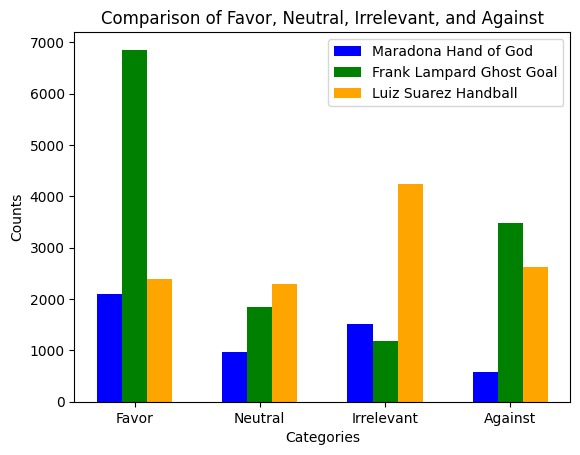
\includegraphics[width=\textwidth, keepaspectratio]{tableonechart.jpg} % Adjust width as needed
        \caption{Number of \textit{Favor}, \textit{Neutral} and \textit{Against} labels}
        \label{fig:labels}
    \end{minipage}\hfill
    \begin{minipage}{0.48\textwidth}
        \centering
        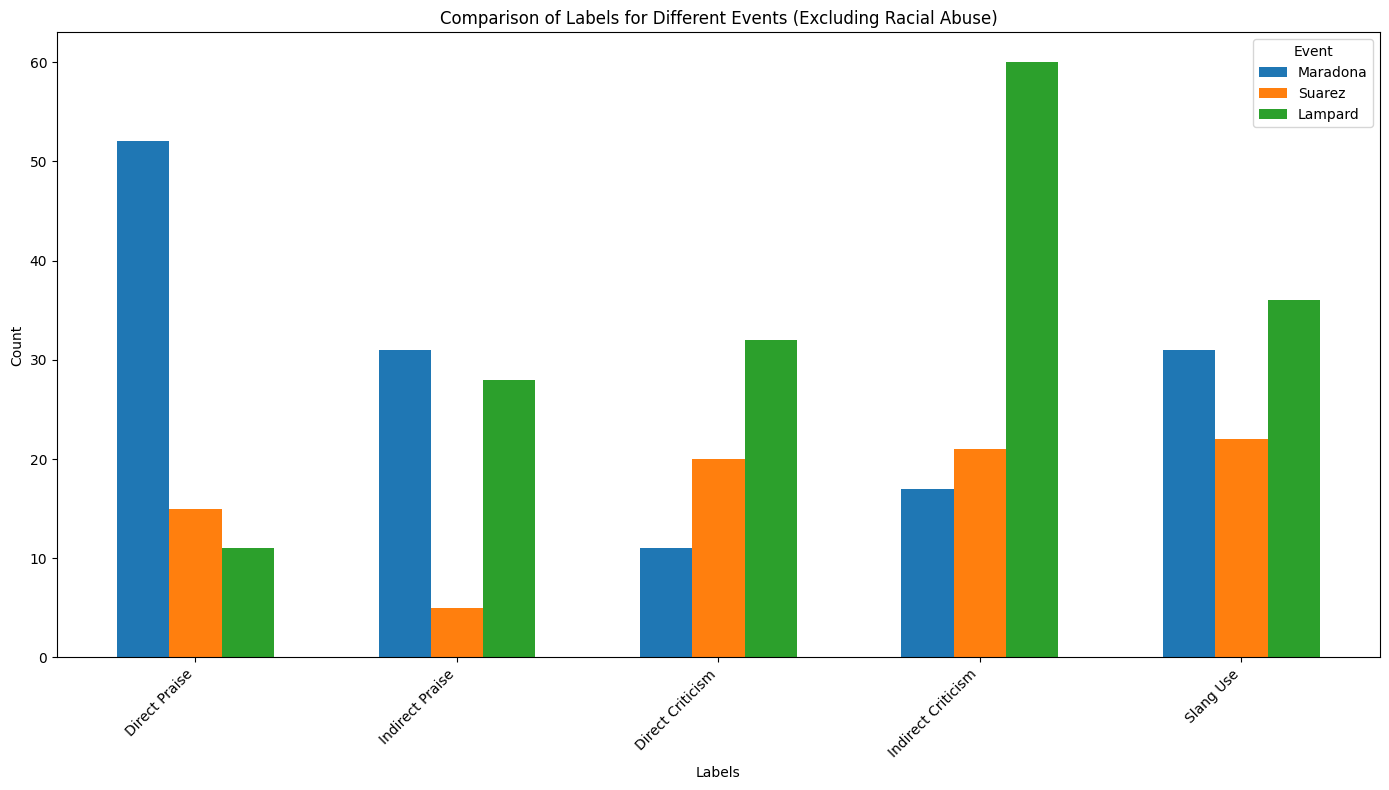
\includegraphics[width=\textwidth, keepaspectratio]{praise_and_criticism.jpg} % Adjust width as needed
        \caption{Comparison of Types of Praise (Favor) and Criticism (Against) for a sample of 200 comments.}
        \label{fig:praise_criticism}
    \end{minipage}
\end{figure*}


% \vspace{5mm} % Add space before table
% \begin{figure*}[htbp]
%     \centering
%     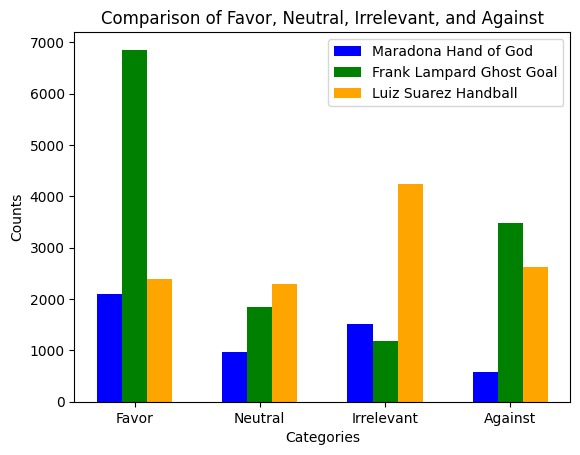
\includegraphics[width=0.8\textwidth, keepaspectratio]{tableonechart.jpg} % Adjust width as needed
%     \caption{Number of \textit{Favor}, \textit{Neutral} and \textit{Against} labels}
%     \label{fig:events}
% \end{figure*}

% \vspace{5mm} % Add space before table
% \begin{figure*}[htbp]
%     \centering
%     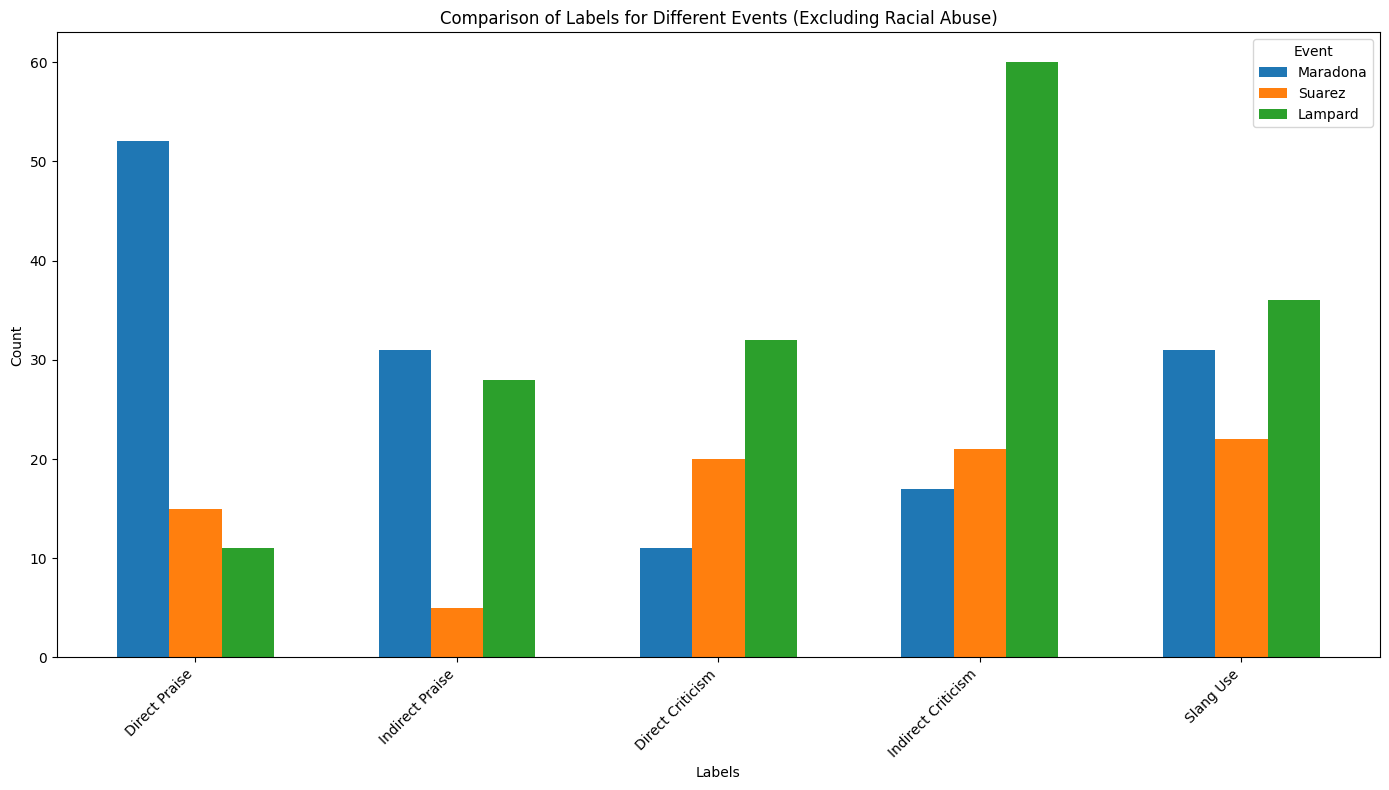
\includegraphics[width=0.8\textwidth, keepaspectratio]{praise_and_criticism.jpg} % Adjust width as needed
%     \caption{Comparison of Types of Praise (\textit{Favor}) and Criticism (\textit{Against}) for a sample of 200 comments.}
%     \label{fig:events}
% \end{figure*}



% \vspace{5mm} % Add space before table

% \begin{table*}[htbp]
%     \centering
%     \begin{tabular}{|c|c|c|c|c|c|}
%         \hline
%         \textbf{Model} & \textbf{Event} & \textbf{Accuracy} & \textbf{Recall (micro)} & \textbf{Precision (micro)} & \textbf{F1 (micro)} \\
%         \hline
%         Llama 3.1-8b-Instruct (Not Fine Tuned) & \textit{Maradona Hand of God} & 46.8\% & 46\% & 56\% & 40\% \\
%          & \textit{Luis Suarez Handball} & 33.7\% & 34\% & 49\% & 24\% \\
%          & \textit{Frank Lampard Ghost Goal} & 26.3 \% & 26\% & 39 \% & 25\% \\
%          \hline
%         Llama 3.1-8b-Instruct (Fine Tuned) & \textit{Maradona Hand of God} & 79.04\% & 79\% & 78\% & 77\% \\
%          & \textit{Luis Suarez Handball} & 79.5\% & 80\% & 79\% & 79\% \\
%          & \textit{Frank Lampard Ghost Goal} & 71.6 \% & 72\% & 72 \% & 72\% \\
%         \hline
%     \end{tabular}
%     \caption{Comparison of models with/without fine-tuning on our constructed dataset}
%     \label{tab:student_info}
% \end{table*}
% % \vspace{5mm}

\subsection{Data Processing}
The extracted comments were preprocessed as follows - 

\begin{enumerate}
 \item Removed special characters, stopwords, and non-English comments. We focussed on the evaluation of mostly English content. 
 \item Irrelevant columns such as nested replies, time of comment and other metadata were removed. 
\item Additional cleaning steps included normalization and duplicate removal, which were essential to enhance the accuracy of the subsequent sentiment and stance analysis.

\end{enumerate}

% Custom footer settings
% \fancyfoot[C]{This is a centered footer}

\begin{table}[h]
    \centering
    \renewcommand{\arraystretch}{0.7} % Increase row height
    \resizebox{0.5\textwidth}{!}{ % Increase table width beyond text width
    \begin{tabular}{|l|r|} 
        \hline
        \textbf{Controversy Name} & \textbf{Number of Comments} \\ 
        \hline
        
        Ashwin Mankading  & 3785  \\  
        % \hline
        Frank Lampard Ghost Goal & 13520 \\
        % \hline
        Johny Bairstow Runout & 6073\\
        % \hline
        Luis Suarez Handball & 11546 \\
        % \hline
        Maradona Hand of God & 5159 \\
        % \hline
        The Underarm Incident & 3676\\
        % \hline
        \hline
    Total & 43759\\
    \hline
    \end{tabular}
    }

   %\captionsetup{justification=centering, font=medium} % Increase font size & center
    \caption{Name of the controversies used and their number of comments. {\color{red}KRIPA: Please put the values.}}
    \label{tab:controversies}
\end{table}


\subsection{Stance Detection Pipeline}
The process for stance detection on our curated dataset constitutes of two stages as follows - 

\begin{enumerate}

\item
    \textbf{Stage-I} (Preparation of "Gold Standard" labels: 
    \begin{enumerate}
        \item \textbf{First pass} - In our first pass, we used an open-sourced LLM from HuggingFace, namely Llama 3.1-8b-Instruct. Custom prompts were constructed for each of the controversies from the dataset along with clear instructions to perform stance detection (for, against, neutral and irrelevant) on the comments for each of these controversies.
        \item \textbf{Second pass} - Subsequently, the generated labels were humanely verified to account for misclassification and/or if further tuning of the prompt was needed to better the distribution of the data.
        \item \textbf{Third Pass} - The tuned few shot prompts were used to perform the stance detection on our dataset and the final labels were generated thereafter.
        
    \end{enumerate}

\item
    \textbf{Stage-II} (Fine Tuning of LLMs on the stance-labeled dataset) : 
    \begin{enumerate}

      \item We used models from the Unsloth library which provides ~70\% reduction in memory usage and up to 2x inference speed.
      \item We chose models like Llama 3.1-8b-Instruct model (same as used for labelling the dataset) to account for the difference made in the metrics when the same model is to be fined-tuned on our dataset.


    \\

    \item Fine tuning on our dataset led to an average increment of ~30\% in terms of accuracy measured and drastic improvement in metrics such as F1, precision and recall as shown by confusion matrix and classification reports compared to its non-fine-tuned model(no data balancing techniques were employed).
    \end{enumerate}

% \\
\end{enumerate}


\\

% \begin{table}[htbp]
% \centering
% \caption{Comparison of Events for Maradona, Frank Lampard, and Luis Suarez}
% \label{tab:events}
% \begin{adjustbox}{width=\textwidth} % Adjust table width to fit the page
% \begin{tabularx}{\textwidth}{l *{6}{X}} % X columns auto-adjust width
% \toprule
% \textbf{Event} & \textbf{Direct Criticism} & \textbf{Direct Praise} & \textbf{Indirect Criticism} & \textbf{Indirect Praise} & \textbf{Slang Usage} & \textbf{Racial Abuse} \\
% \midrule
% \textbf{Maradona} & 12 & 45 & 23 & 34 & 10 & 5 \\
% \textbf{Frank Lampard} & 8 & 50 & 18 & 40 & 7 & 3 \\
% \textbf{Luis Suarez} & 15 & 30 & 25 & 28 & 12 & 8 \\
% \bottomrule
% \end{tabularx}
% \end{adjustbox}
% \end{table}


The following details the above-mentioned pipeline for each of the controversies used to constitute our dataset {\color{red}KRIPA: there should NOT be separate strategies for different events. If it is done, it needs to be justified}. - 
\\

\subsubsection{The Underarm Incident}
For the Underarm Incident, we employed a fine-tuned LLaMA-3 model from Unsloth. A structured prompt was used to classify comments into four categories: \textbf{For, Against, Neutral,} and \textbf{Irrelevant}. The responses were returned in a JSON format and then parsed to extract the stance label and the underlying rationale.

We followed the above-mentioned process for the \textit{Maradona Hand of God} event, \textit{the Luis Suarez Handball} Event and the \textit{Frank Lampard Ghost Goal} Event.
\\

\subsubsection{Jonny Bairstow's Run-Out and Ashwin's Mankadding Events Using the OLLAMA Framework}
For Jonny Bairstow's Run-Out Incident and Ashwin's Mankadding Event, we utilized the OLLAMA framework. Detailed API requests were sent with prompts explaining the context of each event, and JSON responses were parsed to extract the stance label and associated reason. 

% The full code details for this approach are available in the repository: \texttt{[Insert Repository Link]}.


\vspace{5mm} % Add space before table




\begin{table*}[htbp]
    \centering
    \resizebox{\textwidth}{!}{%
        \begin{tabular}{|c|p{4cm}|p{4cm}|p{4cm}|}
            \hline
            \textbf{Event} & \textbf{Favor} & \textbf{Against} & \textbf{Neutral} \\
            \hline
            \multirow{3}{*}{\textit{Frank Lampard Ghost Goal}} 
            & 1. Germans can't say anything about unsporting behavior.  & 1. The 1966 ghost goal had to be paid for. & 1. This was way more clear-cut than 1966. \\
            & 2. What a disgrace this Manuel is.  & 2. Payback for the 1966 final & 2. Inconclusive! Just couldn’t get a good angle. \\
            & 3. Could have been one of the greatest games.  & 3. Even Geoff Hurst said his goal didn’t count. & 3. I remember this game. \\
            \hline
            \multirow{3}{*}{\textit{Luis Suárez Handball}} 
            & 1. Morality always loses, and nice guys finish last.  & 1. Suárez cost Ghana the World Cup semi-final. & 1. He will never step foot in Ghana. \\
            & 2. I just love Luis Suarez with all his behaviors I don't know why.  & 2. This man was often mentally unstable. & 2. That was back then, now there’s goal-line technology. \\
            & 3. By apologizing, he would look stupid. & 3. Hand of Satan. & 3. It’s part of the game. \\
            \hline
            \multirow{3}{*}{\textit{Maradona Hand of God}} 
            & 1. Yup. Goalies s*cked these days. & 1. Errrrr! Hand of god? Cheater. & 1. When the football was football. \\
            & 2. The Real OG of all times. & 2. He makes the opponent look so stupid and clumsy. & 2. Back in the day nobody could play football, that's why he appeared to be that good. \\
            & 3. Number 15 goal is something else...my favourite. Bravo. & 3. The most cheating player in football history. & 3. You will never be able to pick one between Maradona and Messi. \\
            \hline
            \multirow{3}{*}{\textit{Jonny Bairstow Run-Out}} 
            & 1. That's not cheating, that's the way of winning.  & 1. Same old Aussies, always cheating. & 1. The lesson for the players is "pay attention." \\
            & 2. They gave Jonny ample time to stop walking out of his crease, so fair game! & 2. Australia cheating again. Who could have seen that coming? & 2. Growing up in Australia, we were taught to throw the ball at the batters' head if they left their crease like this. \\
            & 3. Jonny was too quick to get out of the crease, so it is totally a fair decision. & 3. Not cheating, just bad sportsmanship. & 3. This is just pure drama and I love it. \\
            \hline
            \multirow{3}{*}{\textit{Ashwin Mankadding}} 
            & 1. If a bowler can keep his foot inside the crease, a batsman can wait with the bat inside the crease until the ball is bowled. What's wrong with that? & 1. If you Mankadding, you should be ashamed of yourself. & 1. Ashwin merely expressed his disappointment but never wanted a wicket that way. \\
            & 2. This is out according to the rule. & 2. Not a fair runout considering sportsmanship and the spirit of the game. & 2. Whenever a batsman leaves the crease, he gets 1 to 2 ft benefits in running. \\
            & 3. Great presence of mind... genius of the game. & 3. This rule is absurd. How can you be allowed to run out someone without delivering the ball? & 3. Batters don’t do it on purpose; they walk out expecting the bowler to deliver the ball. \\
            \hline
            \multirow{3}{*}{\textit{The Underarm Incident}} 
            & 1. That time, it was legal to bowl underarm according to the rules. & 1. That was against the spirit of the game! Couldn't they just bowl a normal delivery? & 1. What were the exact rules for underarm deliveries back then? \\
            & 2. The bottom line is that there was nothing in the rules at the time saying you can't bowl underarm, so technically, nothing wrong was done. & 2. The greatest cowards in the world... None other than the Aussies. & 2. Carrying on about something decades later as if it's relevant today is the real injustice. \\
            & 3. Well, if they were allowed to do it, then fair play to them. & 3. Poor sportsmanship. & 3. Greatest highlight in cricket history, great footage. \\
            \hline
        \end{tabular}%
    }
    \caption{Examples of Favor, Against, and Neutral Comments for Controversial Events}
    \label{tab:event_comments}
\end{table*}





\vspace{5mm} % Add space before table


\begin{table*}[htbp]
    \centering
    \begin{adjustbox}{max width=\textwidth}
        \begin{tabularx}{\textwidth}{|c|>{\raggedright\arraybackslash}X|>{\raggedright\arraybackslash}X|>{\raggedright\arraybackslash}X|>{\raggedright\arraybackslash}X|}
            \hline
            \textbf{Event} & \textbf{Direct Praise} & \textbf{Indirect Praise} & \textbf{Direct Criticism} & \textbf{Indirect Criticism} \\
            \hline
            \multirow{3}{*}{\textit{Maradona Hand of God}}
             & 1. Maradona is sooo good.
             & 1. 13 was simply incredible.
             & 1. 3 was handball. Not a goal. A cheat.
             & 1. You forgot to add the hand of God goal. \\[5pt]
            \cline{2-5}
             & 2. 13 was simply incredible.
             & 2. The legend forever.
             & 2. Goal 12 looks like a huge offside.
             & 2. Back when players played for the crowd, not money. \\[5pt]
            \cline{2-5}
             & 3. The legend forever.
             & 3. Back when players played for the crowd, not money.
             & 3. Cheating and poor goalkeeping.
             & 3. Maradona’s skill ended when he cheated. \\
            \hline
            \multirow{3}{*}{\textit{Luis Suarez Handball}}
             & 1. Suarez is a legend... but seeing Asamoah after the match broke my heart.
             & 1. Suarez took matters into his own hands ����.
             & 1. Suarez crushed so many African dreams.. absolutely criminal.
             & 1. If you watch closely Suarez wasn't even the only one who tried to handball. \\[5pt]
            \cline{2-5}
             & 2. Suarez is a genius.
             & 2. He did what he had to do for his country.
             & 2. Absolute scumbag play.
             & 2. Ghana would have won if it weren't for the handball. \\[5pt]
            \cline{2-5}
             & 3. Suarez hero or villain?
             & 3. Anyone would have done that tho.
             & 3. Suarez will forever be the biggest disgrace in modern football.
             & 3. It's funny though because both Argentina and Uruguay cheated and both got what they had coming. \\
            \hline
            \multirow{3}{*}{\textit{Frank Lampard Ghost Goal}}
             & 1. They were voted the most entertaining team on FIFA.com.
             & 1. It took 12 years but Germany got their karma at last.
             & 1. I hate Germany for what they did, it is so sad.
             & 1.wouldnt have made a difference, im english and we would have lost anyway. German were by far the better team. \\[5pt]
            \cline{2-5}
             & 2. Wouldn't have made a difference, I'm English and we would have lost anyway. Germany were by far the better team.
             & 2. OSCAR winning performance from football.
             & 2. England defended like a bunch of girls.
             & 2. With all the technology today, this would never happen now. \\[5pt]
            \cline{2-5}
             & 3. My idol was Frank Lampard and I'm so happy to see, but that referee was an absolute fuck, blind and should go to the eye doctor.
             & 3. This is the reason why FIFA needs VAR...
             & 3. That's just poor by the officials..smh.
             & 3.The revenge has been taken \\
            \hline
        \end{tabularx}
    \end{adjustbox}
    \caption{Examples of Direct Praise, Indirect Praise, Direct Criticism, and Indirect Criticism }
    \label{tab:maradona_suarez_lampard_comments}
\end{table*}


\begin{table*}[htbp]
    \centering
    \begin{adjustbox}{max width=\textwidth}
        \begin{tabularx}{\textwidth}{|c|>{\raggedright\arraybackslash}X|>{\raggedright\arraybackslash}X|>{\raggedright\arraybackslash}X|>{\raggedright\arraybackslash}X|}
            \hline
            \textbf{Event} & \textbf{Direct Praise} & \textbf{Indirect Praise} & \textbf{Direct Criticism} & \textbf{Indirect Criticism} \\
            \hline
            \multirow{3}{*}{\textit{Maradona Hand of God}} 
             & 1. Maradona is sooo good.  
             & 1. 13 was simply incredible.  
             & 1. 3 was handball. Not a goal. A cheat. 
             & 1. You forgot to add the hand of God goal. \\[5pt]
            \cline{2-5}
             & 2. 13 was simply incredible.
             & 2. The legend forever.
             & 2. Goal 12 looks like a huge offside.
             & 2. Back when players played for the crowd, not money. \\[5pt]
            \cline{2-5}
             & 3. The legend forever.
             & 3. Back when players played for the crowd, not money.
             & 3. Cheating and poor goalkeeping.
             & 3. Maradona’s skill ended when he cheated. \\
            \hline
        \end{tabularx}
    \end{adjustbox}
    \caption{Examples of Direct Praise, Indirect Praise, Direct Criticism, and Indirect Criticism for Maradona Hand of God}
    \label{tab:maradona_comments}
\end{table*}





\vspace{5mm} % Add space before table

\begin{table*}[htbp]
    \centering
    \begin{tabular}{|c|p{12cm}|}
        \hline
        \textbf{Event} & \textbf{Example Comments} \\
        % \hline
        \multirow{9}{*}{\textit{Frank Lampard Ghost Goal}} 
         & \textbf{Favor} \\
         & 1. I wonder what Germans think to unsporting behaviour. They don't think. ������ \\
         & 2. What a disgrace this Manuel is. \\
         & 3. Could had been one of the greatest games of all time but ref decided, no…. \\
         \hline
         & \textbf{Against} \\
         & 1. Even Geoff Hurst in 1966 said my goal didn’t count even though it was a goal. This is just revenge, I believe. \\
         & 2. Geoff Hurst's "ghost" winning goal in 1966 had to be paid.  
           1970 - Losing the QF to Germany after leading 2-0.  
           1990 - Losing the semi-final on penalties.  
           2010 - Lampard’s goal not seen by the assistant referee.  
           The curse started right after the final whistle of the 1966 World Cup Final. \\
         & 3. Payback for the 1966 final ���� \\
         \hline
         & \textbf{Neutral} \\
         & 1. Inconclusive! Just couldn’t get a good angle on that. \\
         & 2. Didn’t cross the line. \\
         & 3. Not enough evidence to overturn the decision. \\
        \hline
    \end{tabular}
    \caption{Example sentiment-based comments for Frank Lampard's Ghost Goal event}
    \label{tab:frank_lampard_comments}
\end{table*}




\subsection{Algorithm Details and Rationale}
The following outlines the overall pipeline and reasoning behind our stance detection approach:
\begin{itemize}
    \item \textbf{Pipeline Design:} The pipeline starts with data extraction and preprocessing to ensure the quality of the input comments. Given the noisy nature of social media data, thorough cleaning was essential.
    \item \textbf{Model Selection:} For the Underarm Incident, the fine-tuned LLaMA-3.1 (Instruct) family of models were chosen for its ability to process long sequences (up to 2048 tokens) and follow the given instructions (as a few shot prompts) to generate coherent responses, making it suitable for detailed stance detection.
    \item \textbf{Structured Prompts:} We used structured prosmpts to guide the model in classifying comments. This method provided consistent JSON responses, ensuring ease of parsing and reliable extraction of stance labels and reasons.
    \item \textbf{OLLAMA Framework:} For Jonny Bairstow's and Ashwin's events, the OLLAMA framework allowed for scalable and concurrent processing of comments via API calls. This was critical in handling larger datasets and ensuring a rapid turnaround in analysis.
    \item \textbf{Evaluation Metrics:} In addition to the stance labels, we compute evaluation metrics such as accuracy, precision, recall, and F1-score to assess model performance.
\end{itemize}



Figure~\ref{fig:pipeline} presents a flowchart summarizing the stance detection pipeline.




\begin{figure}[ht]
\centering
\includegraphics[width=0.48\textwidth]{pipeline_flowchart.png}  % Replace with your actual flowchart image
\caption{Stance Detection Pipeline Flowchart}
\label{fig:pipeline}
\end{figure}

For clarity, the pseudocode in Algorithm~\ref{alg:pipeline} summarizes the pipeline:

\begin{algorithm}[h]
\caption{Stance Detection Pipeline}
\label{alg:pipeline}
\begin{algorithmic}[1]
\STATE \textbf{Input:} YouTube comments dataset
\STATE \textbf{Preprocessing:} Clean comments by removing noise and duplicated data
\IF{Incident is Underarm}
    \STATE Use the Unsloth LLaMA-3(Instruct) family of models with a structured prompt
    \STATE Parse JSON response to extract stance label and reason
\ELSE
    \STATE Use the OLLAMA framework with API requests and detailed prompts
    \STATE Parse JSON response to extract stance label and reason
\ENDIF
\STATE \textbf{Output:} Stance labels and evaluation metrics (accuracy, precision, recall, F1-score)
\end{algorithmic}
\end{algorithm}

\section{Results and Discussion}

Preliminary analysis indicates a significant division in public opinion across the six events within our dataset. 
Fine Tuning on our dataset improves the accuracy of the labels by a drastic margin along with other metrics such as F1 score, recall and precision as compared to the base instruct model.

Detailed results, including the distribution of stances (For, Against, Neutral, Irrelevant) and evaluation metrics (accuracy, precision, recall, F1-score).


\subsection{Detailed Analysis}
\begin{enumerate}
    \item \textit{Number of samples} (\textbf{Favor}, \textbf{Against}, \textbf{Neutral} and \textbf{Irrelevant})
    \begin{enumerate}
    \item The labels, \textit{Favor} and \textit{Against} is significantly higher for  \textit{Frank Lampard Ghost Goal} compared to other events with \textit{Favor} being comparatively higher, followed by \textit{Luiz Suarez Handball} event.
    \item The \textit number of samples for {Neutral} label is higher for \textit{Luis Suarez Handball} event.
    \item The label \textit{Irrelevant} is significantly higher for \textit{Luis Suarez Handball} event meaning the majority of the comments couldn't be classified into the other three labels.
    \end{enumerate}
    \item \textit{Variations of Praise and Criticism}
    \begin{enumerate}
        \item Instances of \textit{Direct Criticism} and \textit{Racial Abuse} is highest for \textit{Maradona Hand of God} event.
        \item \textit{Direct Praise} accounts highest for \textit{Luis Suarez Handball} with equal instances for \textit{Maradona Hand of God} and \textit{Frank Lampard Ghost Goal}.
        \item For \textit{Indirect Criticism}, \textit{Frank Lampard Ghost Goal} is highest followed by \textit{Maradona Hand of God}.
        \item In terms of \textit{Favor} label (Direct + Indirect Praise), Frank Lampard event is highest, followed by Maradona and then by Luis Suarez events.
        \item  Similarly, for \textit{Against} label (Direct + Indirect Criticism), Maradona event's count is highest followed by Frank Lampard and then Luis Suarez events.
    \end{enumerate}


      \item \textit{Fine Tuning of LLMs}
    \begin{enumerate}
        \item Without fine-tuning, Llama3.1-8b Instruct got an average of 35.6 \% and with fine-tuning on our constructed dataset, there was a drastic improvement of over 40 \% to 76.71 \%.
        \item This improvement is majorly due to the quality of labels associated with the respective comments after a thorough human verification.
       
    \end{enumerate}
    
    
\end{enumerate}

\subsection{Challenges Encountered}
During preprocessing, challenges such as handling noisy data, duplicate entries, and variations in comment formats were encountered. For stance detection, ensuring reliable automated classification and consistent JSON parsing proved difficult. These challenges motivated the use of structured prompts and robust frameworks like OLLAMA.

\subsection{Future Directions}
Future work will focus on:
\begin{itemize}
  \item Refining sentiment classification models using advanced machine learning techniques.
  \item Expanding the dataset to include a broader range of sports controversies.
  \item Enhancing preprocessing methods and fine-tuning model parameters to improve overall performance.
\end{itemize}

\section{Ethical Considerations}
In this study, the ethical use of publicly available YouTube data was ensured. All data were anonymized and processed in accordance with ACM's policies on research involving human subjects. Informed consent was addressed by using publicly accessible data without any direct identification of individuals.

\section{Conclusion}
This study highlights the role of social media in shaping public perception of sports controversies. The integration of automated data extraction and stance detection provides a comprehensive view of audience sentiment. Future enhancements will aim to improve accuracy and broaden the scope of analysis.

%%
%% The next two lines define the bibliography style to be used, and
%% the bibliography file.
\bibliographystyle{ACM-Reference-Format}
\bibliography{sample-base}


%%
%% If your work has an appendix, this is the place to put it.

\end{document}
\endinput
%%
%% End of file `sample-sigconf.tex'.
